%!TEX root = ../main.tex
%%%%%%%%%%%%%%%%%%%%%%%%%%%%%%%%%%
% Links:
%
% Difficulty: Easy/Medium Companies: 
%%%%%%%%%%%%%%%%%%%%%%%%%%%%%%%%%%

%\chapterimage{header}

\chapter{Power set generation}
\label{ch:power_set}
\section*{Introduction}

The concept of power set is familiar to many because it is one of the topics of the first
introductory math courses on set theory.

The power set of a set $S$ is the set of all its subsets and in this lesson, we will explore how we can generate the power set of a given set. Very often this is a task we are challenged to solve directly as well as indirectly as part of a coding interview question.

We will investigate two different approaches to solve this problem: 

\begin{enumerate}
    \item The first derives straightforwardly from the recursive definition of power-set which says that the power-set of an empty set is a set containing one element only: the empty set itself. 
    For a non-empty set $S$, let $e$ be an element of $S$ and $T$ be the original set $S$ set minus $e$ ( $T=S \setminus e$), then the power set of $S$ is defined as the union of two distinct power sets:
    \begin{itemize}
        \item   the power set of $T$
        \item   and the power set of $T$ modified in a such way that $e$ is added to all of its elements. 
    This idea is formalized in the Equation \ref{eq:power_set_recursive_definition}:

    $\mathcal{P}(S)=\begin{cases} 
        \{\{\}\} & \text{if } S=\{\} \\
        \mathcal{P}\{T\} \bigcup \{t \bigcup \{e\} \: : t \in \mathcal{P}\{T\}\} \text{ where }  T = S \setminus \{e\} \text{ } \forall e \in S, & \text{otherwise}
        \end{cases}$
    \end{itemize}
    
    \item The second is based on a property of the distribution of the bits in the binary representation of the integers from $0$ to the size of the
    power set. 

\end{enumerate}




\section{Problem statement}
    \begin{exercise}
        Write a function that given a set $S$ returns its power set.
The power-set of $S$ ($\mathcal{P}(S)$) is the set of all its subsets including the empty subset ($\emptyset$) and $S$ itself.

        \begin{example}
            \label{ex:power_set:example1}
            \hfill \\
            Given the set $S=\{a,b,c\}$, the following is a correct output for
            this problem: $$\{\{\}, \{a\}, \{b\}, \{c\}, \{a,b\}, \{b,c\}, \{a,c\}, \{a,b,c\} \}$$
        \end{example}
    \end{exercise}

\section{Clarification Questions}

\begin{QandA}
    \item What is the maximum input size?
    \begin{answered}
        \textit{The maximum number of element in $S$ is strictly less than $32$.}
    \end{answered}
    
    \item Are all the elements in the collection distinct?
    \begin{answered}
        \textit{No, the elements are not necessarily distinct. $S$ might contain duplicates..}
    \end{answered}

    \item Can the elements of the power-set appear in any order?
    \begin{answered}
        \textit{Yes, subsets can appear in any order. 
        For example the following is also a valid output for the input shown in Example \ref{ex:power_set:example1}:} 
        $\{\{\}, \{b,c\}, \{a\}, \{a,b\}, \{a,b,c\}, \{b\}, \{a,c\}, \{c\} \}$
    \end{answered}
\end{QandA}

\section{Discussion}
\label{sec:powerset:discussion}

There is one key point that should immediately be noticed: The power set of a collection of $n$ elements has size $2^n$. The proof  is relatively easy, and it boils down to the fact that a subset of $S$ can be uniquely identified by a list $X=\{x_0,x_1,\ldots x_{|S|-1}\}$ of $|S|$ binary variables each carrying the information about whether $S_i$ is part of the subset; $x_i$ answers the question: \textbf{should $S_i$ be part of this subset?} If $x_i$ is true the answer is yes, otherwise it is no. Because we have two possible choices for every element of $S$ (either take it or not), then the total number of distinct $X$s  is: $2 \times 2 \times \ldots \times 2 = 2^{|S|}$. Two choices for the first element, two for the second, and so on until the last element of $S$.
  
This, together with the constraint on $|S|$ ($|S| < 32)$ is a strong hint towards the fact that an \textbf{exponential time and space} solution is expected.
After all, we are required to output all the elements of the power set, and thus the number of operations of an algorithm designed for this task cannot be less than the size of the power set itself. 


\subsection{Bruteforce - Backtracking-like approach}


The first solution presented in this lesson is based on the fact that  during the generation of one of the elements of the power set a decision has to be taken for each element $e$ of $S$, on whether to include or not $e$ into the subset. 
When a decision for the first element is taken, we are left with are $|S|-1$ decisions
before we have created a valid subset of $|S|$.

This kind of process is inherently recursive and is easily visualized with a tree (see the Figure \ref{ref:power_set_decision_trees}) where a node at level $i$ represents a decision for the $i^{th}$ element of $S$ and a path from the root to a leaf uniquely identifies a subset of $S$ as, after having traversed all the levels down to a leaf, $n$ decisions have been taken: one for each of the elements of $S$. 
Collectively, all the paths from the root to the leaves are the power set, and therefore, in
order to solve this problem, we have to visit the entire tree.


A general way to deal with such type of problems is by using a backtracking-like approach to try all possible
decisions (or equivalently to visit every path from the root to a leaf).
The idea is that, for all elements of $S$, from first to last, we are going to
explore the two available possibilities: either take or exclude the
it from the subset.

We start by making a decision for the first element and continuing from there to generate all possible subsets
where the first decision is never changed. 
When there are no more subsets to generate, we \textit{backtrack} and change our first
decision and repeat the process of generating all possible subsets.

For instance, given $S=\{1,2,3\}$, we might start by deciding to use the element $1$, and include it in all possible subsets from the remaining elements $\{2, 3\}$ only. 
When we are done with it we can repeat the same process, only this time, excluding $1$. What we do is: $\mathcal{P}(S)= \{\{1\} \; \bigcup \;\mathcal{P}(\{2,3\})\} \: \bigcup \: \{\mathcal{P}(\{2,3\})\}\} 
$

The proposed solution will incrementally construct one subset at a time, 
using an integer variable to keep track of which element we are currently taking the decision for.
This type of problem is naturally solved recursively, with a base case of the recursion happening when there is no more decision
to take, meaning that the current subset is ready to be included in the solution (it has been
produced after $n$ decision steps).

The C++ code implementing the idea above is shown in Listing \ref{list:power_set_backtracking}. The complexity of this solution is exponential i.e. $O(2^n)$ which as already pointed out is as good as
it gets.


\lstinputlisting[language=c++, caption="C++ to the power set generation using backtracking",label=list:power_set_backtracking]{/home/dspataro/git/algorithm_articles/sources/power_set/power_set_backtracking.cpp}




\begin{figure}
    \centering
    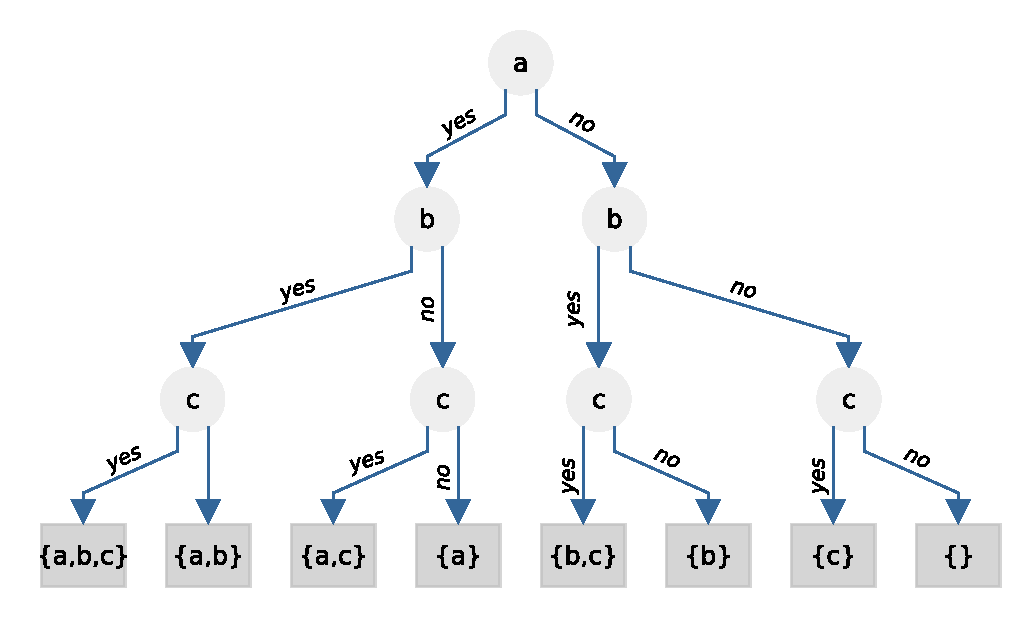
\includegraphics[width=\textwidth]{/home/dspataro/git/algorithm_articles/sources/power_set/images/tree}
    \caption[Decision tree for the power-set generation using backtracking.]{Decision tree for the power-set generation using backtracking. At level $i$ are the decision for the element $i$ in the original set. A label marked with yes identifies the decision to take the corresponding element into the subset, while a node labeled with no the opposite. At the last level is the power set.}
    \label{ref:power_set_decision_trees}
\end{figure}

The advantages of using this backtracking-like approach to solve this problem are that, once we notice
that a problem can be solved by fully exploring the associated search space tree, then we can immediately
start writing the code and rely on our experience as backtracking expert writers to implement a correct
solution with the added bonuses of being concise and short when written in a recursive  form (which gives you fewer chances to make mistakes, and less code to debug and explain),  as well
as well understood.
The downside is that, if you decide to go for it, an iterative implementation can be a little harder and more verbose to write.

Regardless of which type you decide to write, the interviewer is going to be pleased with your code provided you get to the final solution
without making too many implementation mistakes like forgetting to handle the base case.

\subsection{Bit Manipulation}

Another approach that can be used to solve this problem is based on the fact that the values of the
bits of the numbers $\{0,1,2,\ldots, s^n-1\}$  already provide all the information necessary to decide whether to include or not an element from $S$ into a subset. 
The main idea is that the binary representation of all the numbers ($2^{|S|}$ of them) from $0$ to $2^{|S|}-1$ is the power set of $n$ bits.
This practically means that the binary representation of any of those numbers carry the necessary information that can be used to build one subset of $\mathcal{P}(S)$. 


For instance for the input $S=\{a,b,c\}$ the Table \ref{tab:mapping_value_bits} shows numbers from $0$ to $2^3-1 = 7$ and their binary representation (in the second column) as well as how the information about which bit is set can be used to construct one
subset of $\mathcal{P}(S)$ (in the third column).
\textbf{When the $i^{th}$ bit is set (its value is $1$), it means that
corresponding $i^{th}$ element of $S$ is chosen, while an unset bit (with value $0$) means it is
excluded}.


\begin{table}
    \centering
    \begin{tabular}{|l|l|l|}
        \hline
        Number Value & Bits & Subset\\ \hline
        0     & 000  & $\{\}$\\ \hline
        1     & 001  & $\{c\}$\\ \hline
        2     & 010  & $\{b\}$\\ \hline
        3     & 011  & $\{b,c\}$\\ \hline
        4     & 100  & $\{a\}$\\ \hline
        5     & 101  & $\{a,c\}$\\ \hline
        6     & 110  & $\{a,b\}$\\ \hline
        7     & 111  & $\{a,b,c\}$ \\ \hline
    \end{tabular}
    \caption[Mapping between bits and element of the power set.]{This table shows a 1-to-1 mapping between integer values, their binary representation and an element of the power set.}
    \label{tab:mapping_value_bits}
\end{table}


This idea can be used to write an algorithm in which all the numbers in the range $\{0,1,2,\ldots,
2^{|S|}-1\}$ are considered and each of them is used to generate a subset of the final solution.
Every number from this range maps uniquely to a subset of $\mathcal{P}(S)$. 

It is not
surprising when we think about the meaning of a bit in the binary representation of integers. One
can "build" a number $k$ by summing up powers of $2$ where the bits contain the information about whether a
certain power of two should be added to the final value. With $n$
bits one can represent $2^n$ numbers, each corresponding to one and only one subset of the power set of those $n$ bits.


Listing \ref{list:power_set_bits} shows  a possible C++ implementation of the idea above.


\begin{lstlisting}[language=c++, caption=Binary tree definition used in this exercice.,label=list:verify_BST:tree_structure]

    struct TreeNode {
        int val;
        TreeNode *left;
        TreeNode *right;
        TreeNode(int x) : val(x), left(nullptr), right(nullptr) {}
    };
    \end{lstlisting}


The complexity of this function is, not surprisingly, $O(2^{|S|})$. 
We also pay a constant price of $32$ for each number we loop through since we need to inspect all of its bits.
The proposed implementation assumes that the size of \inline{int} is $4$ bytes, 
which is true for most systems.

Moreover, notice the usage \inline{std::reserve}
that should be used in all those scenarios when we already know the final size of the
collection we are building. This saves time because avoids intermediate allocations and copies that must happen during the resize of the vector.






%\section{Common variations}

%\section{Conclusion}
